\documentclass[12pt]{paper}

\usepackage{Schwieg}
\usepackage[margin=1in]{geometry}
\usepackage{tikz}

\begin{document}


\author{Daniel Noriega \and Timothy Schwieg \and Samuel Barker \and
  Rafeh Qureshi }
\title{Problem set 5 - Question 2}

\maketitle

\section*{Model}

Each supplier combines labor $\ell$ and capital $k$ to form output $y$
that is sold at price $p$. Each firm can produce at most output $y =
1$ but can choose to produce $0$ or anything in between. Assume that
each firm has decreasing returns to scale, i.e. marginal cost is
increasing in output.

Firms are indexed by their technology, with firm $i$ having production
function $f_i (k, \ell)$. The profit maximization problem that faces each
firm is:
\begin{align*}
  \max_{\ell,k} \quad& p f_i (k, \ell ) - w \ell - r k\\
  \text{s.t.} \quad & f_i ( k, \ell ) \leq 1
\end{align*}

Each firm faces the typical cost function:
\begin{align*}
  C( w, r, y ) = \min_{\ell,k} \quad & w \ell + r k\\
  \text{s.t.} \quad & f_i ( k, \ell ) = y
\end{align*}

With the simple restriction that output $y$ cannot be greater than
$1$. This yields a cost function $C_i ( w, r, y)$ for each firm that
will be used in the analysis.

Note that it is not the case that firms are not earning profits in
this industry. The firms with the better technology, in the sense that
their cost is lowest for a given level of $w,r$ are able to produce
their output for less money than its more costly competitors.

There are always some firms that are on the margins, these firms are
indifferent between exiting the market and staying in, meaning that
they are earning zero profits. These firms have the worst technology
for the given costs of the factor inputs. Firms with ``better''
technology, their costs are less for the given factor costs all make
positive profits.

\section*{Describe how an individual firm's factor demands vary with
  the output price and the factor rental rates}

There are three cases of interest for the firms in this industry. For
some fixed cost of factor inputs, each firm must lie in one of these three
categories.

\subsection*{Firm Chooses not to enter the market}

For the given cost of the factor inputs, for any level of output, the
firm's in this category face costs that are higher than its revenue, i.e.,
$py < c( w, r, y) \quad \forall y \in (0,1]$. These firms have factor demands of
zero, and some of them have such high costs compared to the price, that any
differential change to the factor prices would not cause them
to enter the market. This case is rather trivial as they will
always have factor demands of zero--even after a price change.

Another possibility is the firm finds its profit maximizing choice of
output is $0$ units of output. If there is a differential change in
the output price, it is possible that these firms will decide to
enter the market. This choice of whether or not they will choose to
enter the market is determined by the sign of $p - C_y(w,r,0)$, if
this number is positive, the firm finds positive profit from entering
the market, and will produce to the value of $y \in (0,1)$ where $p =
C_y(w,r,y)$. This value of $y$ will be
denoted $y^{*}$. The factor demands would then be given by the
solutions to

\begin{align*}
  \deriv{f_i(\ell,k)}{\ell} &= \frac{w}{p}\\
  \deriv{f_i(\ell,k)}{k} &= \frac{r}{p}
\end{align*}

These determine the values of $\ell^{*}$ and $k^{*}$ that maximize profit
for the firm.

\subsection*{Firm Enters the Market, but Output Constraint is not
  Binding}

These firms can be split into two segments, the firms that are
producing output in the interior of $(0,1)$ and the firms that are
producing output of $y=1$ but would choose to produce at that level
regardless of the constraint.

The interior producing firms will react according to the traditional
view of factor inputs. They will demand $\ell^{*}, k^{*}$ such that
\begin{align*}
  \deriv{f_i(\ell,k)}{\ell} = \frac{w}{p}\\
  \deriv{f_i(\ell,k)}{k} = \frac{r}{p}
\end{align*}

The output that each firm produces will be given by:
$y^{*} = f(\ell^{*}, k^{*})$. When a factor input changes, these firms
will see a substitution and a scale effect. When the price changes,
the firms compensate by producing more output so that $p = C_y$. As
marginal cost is increasing in $y$ this means that they produce
strictly more output. This means that they will use more of at least
one input.  As factor input prices drop, the firm consumes more of
this input, as both the substitution and the scale effect lead to
higher usage. Whether or not it consumes more or less of the other input
is related to the technology of the firm.

The interesting case occurs for the firms that are choosing to produce
at output $y = 1$. These firms are not able to ramp up their
production when factor prices are reduced, and so realize higher profits--revenue is the same, but costs are lower.

They may be able to substitute the cheaper input for the relatively more expensive input, but cannot choose to produce more output. Thus, an increase in the output price has no effect on how much these firms produce, because they cannot choose to raise their output past (in particular, at $y=1$). Fortunately, because these firms may be able to choose a less costly mix of inputs after the price of one factor falls, they are able to achieve greater profits than they were before. Even if they did not choose to switch up the mix of inputs, they would still experience higher profits. To see this, suppose that they do not make higher profits. This is obviously impossible since they are experiencing the same costs (under the assumption that they did not change production at all), but are able to sell at higher prices. \textbf{Thus profits for these firms always increase, and output remains the same since the constraint becomes binding.}


\subsection*{Output Constraint is binding for the firm}

These firms are facing the output constraint binding--similar to the last case above, but they are not \textit{choosing} to produce at $y=1$. They produce
output at level $y^{*} = 1$ and are making positive profits. We know that they are making positive profits, because they are constrained. Price
changes have no impact on the firms factor demands (because this is determined in the cost function), as any
differential change results in the firm continuing to have positive
profits and produce at $y^{*} = 1$.

When the factor rental rates change, there is still a substitution
effect for the firms undergone in the cost function. The firms still
choose to produce where $y=1$ but the optimal levels of $\ell^{*}$ and
$k^{*}$ are not fixed. These amounts will change as the relative costs
of $\ell$ and $k$ change. As the price of a factor input decreases, more
of that input will be used, but depending on the technology,
less of the other input would be demanded.

\section*{If the suppliers were using the two factors in fixed
  proportions, what is the relationship between the industry's factor
  demand the individual producer's factor demands?}

We take ``fixed proportions" of factor usage to mean Leontief technology (as was given in an earlier problem set). This means
that the two inputs are perfect complements, and we can write the
technology that each firm has as $f_i(\ell,k) = \alpha_i \min \{ \ell, \beta_i k
\}$. Firms differ on two fronts, the proportion of capital that gets
combined with labor, and the output produced by a combination of one
unit of labor and $\beta_i$ units of capital. Note that this function
displays CRS, so marginal cost is independent of output level.

\begin{align*}
  C(w,r,Y) &= \min_{\ell,k} w \ell + r k \\
  &\text{s.t.} \quad \alpha_i \min \{ \ell, \beta_i k \} = Y
\end{align*}

This yields a solution of:
\begin{equation*}
  C(w,r,Y) = Y \left( \frac{w}{\alpha_i} + \frac{r \beta_i}{\alpha_i} \right)
\end{equation*}

This is just a line, and therefore its marginal cost is constant. Using the
profit maximizing condition of $p = MC$, when the price is above the
marginal cost, the firm will produce $1$ unit; and, when it is equal,
the firm is indifferent between all production, so assume it produces
$1$ unit. When it is below, the firm chooses not to produce.

This means the only choice that a firm faces is whether or not to be
in business or not, and if it is in business, it produces $1$ unit of
output. This allows us to construct the factor demand
equations from the unconditional ones. Note that $\indicate{.}$ is an
indicator function returning $1$ if the inside condition is true, and
zero otherwise.
\begin{align*}
  \ell^{*} &= \frac{1}{\alpha_i} \indicate{ p \geq \left( \frac{w}{\alpha_i} + \frac{r
  \beta_i}{\alpha_i} \right)}\\
  k^{*} &= \frac{1}{\beta_i \alpha_i} \indicate { p \geq \left( \frac{w}{\alpha_i} + \frac{r \beta_i}{\alpha_i} \right)}
\end{align*}


The industry's factor demand equations are simply the sum of these
factor demand equations. This can be simplified by realizing for fixed
factor input prices, the firms in the industry can be ordered
according to their marginal cost.

For a set of isoquants for the production of one unit of output, and
given input prices, one isoquant produces them at lowest cost. we say
this is the lowest cost isoquant for these factor input prices. This
can be seen in the graph below.
% Insert a picture of various isoquants and price lines

$$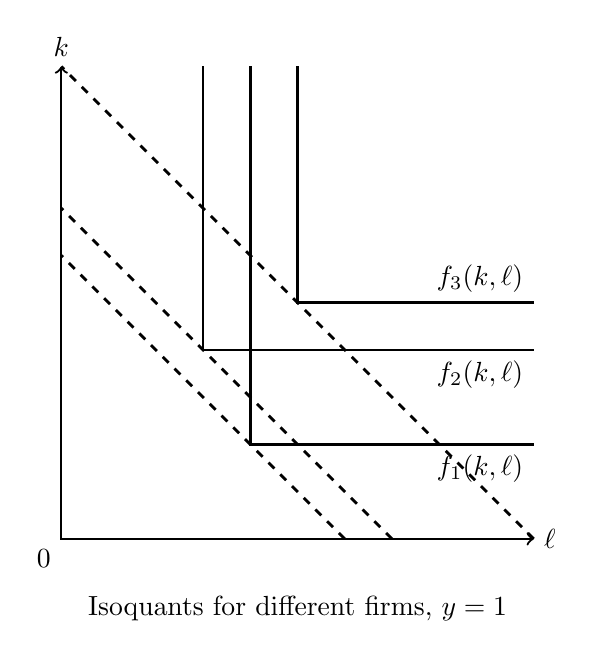
\begin{tikzpicture}[scale=0.6, line width = 1pt]

\draw[thick,<->] (0,10) node[above]{$k$}--(0,0)--(10,0) node[right]{$\ell$};

\node [below left] at (0,0) {$0$};

\draw (10,4)--(3,4)--(3,10);
\node [below left] at (10,4) {$f_2(k,\ell)$};
\draw (10,2)--(4,2)--(4,10);
\node [below left] at (10,2) {$f_1(k,\ell)$};
\draw (10,5)--(5,5)--(5,10);
\node [above left] at (10,5) {$f_3(k,\ell)$};

\draw [dashed] (10,0)--(0,10);
\draw [dashed] (7,0)--(0,7);
\draw [dashed] (6,0)--(0,6);

\node [below] at (5,-1){Isoquants for different firms, $y=1$};

\end{tikzpicture}$$


For the set of all the firms, denote firm $1$ by the lowest cost firm
for production of $1$ output. Firm $2$ is then the second lowest, and
so on ordering all the firms. When firms tie, any possible tie-breaker
is valid.

For given input prices, find the highest cost firm that is willing to
produce. All firms with costs below this firm are also willing to
produce. This is the collection of all firms producing. Call this
number $N_{H}$. The industry factor demand equations is then the
sum of all of the individual factor demand equations

\begin{align*}
  \ell_I^{*} &= \sum_{i=1}^{N_{H}} \frac{1}{\alpha_i}\\
  k_I^{*} &= \sum_{i=1}^{N_{H}} \frac{1}{\beta_i \alpha_i}
\end{align*}

As the price of an input changes, this can only affect the industry
demand by making more or less firms enter the market. If the input
price is reduced, some firms may enter the market, and then demand the
inputs required to produce one unit of output. Note that the firms that have technology that more heavily emphasis a factor that has a changing price are more impacted. In other words, if wages fall (rise), firms whose share of labor is higher are more likely to enter (leave) the market than those with lower shares of labor. This comes from the fact that firms with a larger share of labor experience a larger cost reduction (increase) from a fall (rise) in wages.

If an input price
increases, the same effect could happen with firms exiting the
market. If no firms choose to enter or exit the market, changing the
prices can only re-order the firms in terms of lowest cost, which has
no effect on the industry demand.

\section*{What does the cost function look like for this industry?}

The cost function for an individual firm is given by:

\begin{equation*}
  C(w,r,Y) = Y \left( \frac{w}{\alpha_i} + \frac{r \beta_i}{\alpha_i} \right)
\end{equation*}

By the logic used in part (b), there is a rank ordering between the various firms
in terms of cost. Order these firms in such a way. The lowest cost
manner for the industry to produce $1$ unit of output is to use the
lowest cost firm, firm $1$. After firm $1$ is at max capacity, it must
go to the next best alternative, firm $2$, and so on. Each firm has
linear cost, where the slope is increasing between the firms. This
means that the industry cost function is a piece-wise linear function
that is convex.

% Insert picture of this shit.

$$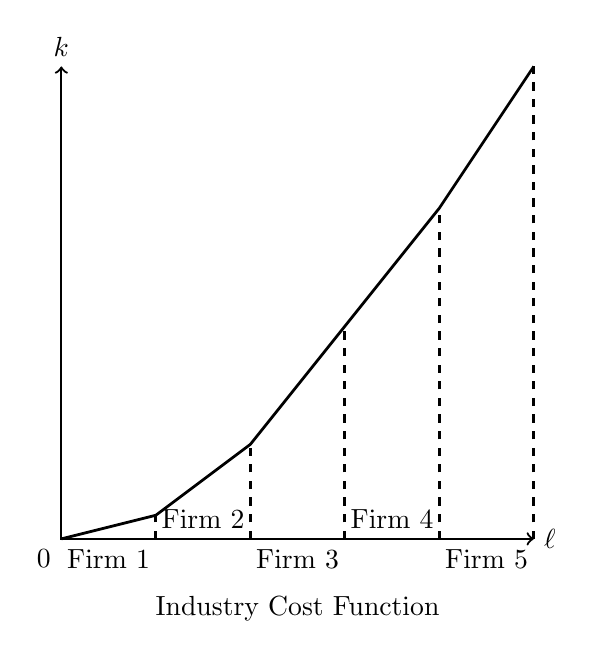
\begin{tikzpicture}[scale=0.6, line width = 1pt]

\draw[thick,<->] (0,10) node[above]{$k$}--(0,0)--(10,0) node[right]{$\ell$};

\node [below left] at (0,0) {$0$};

\draw (0,0)--(2,.5)--(4,2)--(6,4.5)--(8,7)--(10,10);

\draw [dashed](2,0)--(2,.5);
\node [below] at (1,0){Firm 1};
\draw [dashed](4,0)--(4,2);
\node [above] at (3,0){Firm 2};
\draw [dashed](6,0)--(6,4.5);
\node [below] at (5,0){Firm 3};
\draw [dashed](8,0)--(8,7);
\node [above] at (7,0){Firm 4};
\draw [dashed](10,0)--(10,10);
\node [below] at (9,0){Firm 5};

\node [below] at (5,-1){Industry Cost Function};

\end{tikzpicture}$$

\section*{How would your answers be different if the suppliers had no
  production capacity limit}

Since there is still Leontief technology, but now no matter what the
output level is, firm $1$ still produces at minimum cost. He still has
constant returns to scale, so he is different between any amount of
production. This means he will be willing to produce at any output
level. Assume that he will produce at the market clearing level of
output. In this sense, the supply in the entire industry is what this
single firm chooses to supply, as it can always produce at cheaper
cost than any other firm in the business.

However it is not the case that this firm has monopoly power in this
world. If it raises the price to the point that the second least cost
firm can make profits, then that firm will enter the market. This
means that the degree of power that the firm has is related to the
difference in cost between firm $1$ and firm $2$. We assume here that
the costs of firm $2$ are closer to firm $1$ than the monopoly
solution to the problem, namely $MR = MC$.

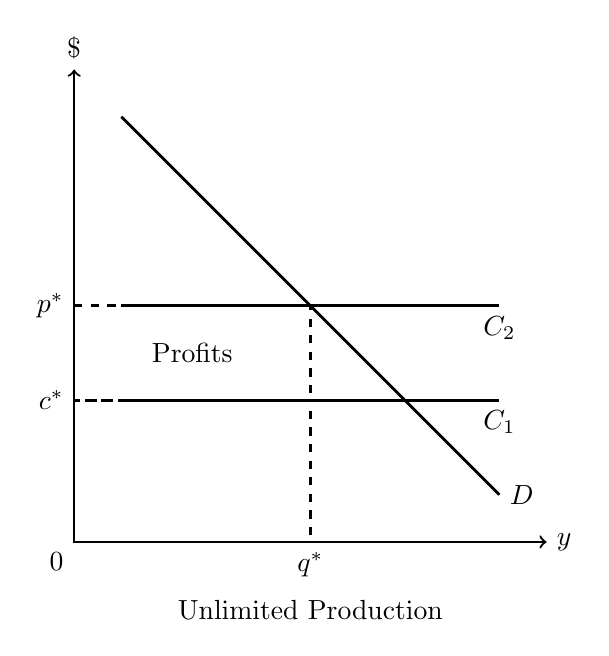
\begin{tikzpicture}[scale=0.6, line width = 1pt]

\draw[thick,<->] (0,10) node[above]{$\$$}--(0,0)--(10,0) node[right]{$y$};

\node [below left] at (0,0) {$0$};

\draw (1,9)--(9,1);
\node [right] at (9,1){$D$};

\draw (1,3)--(9,3);
\node [below] at (9,3){$C_1$};

\draw (1,5)--(9,5);
\node [below] at (9,5){$C_2$};

\draw[dashed](0,5)--(5,5)--(5,3)--(0,3)--(5,3)--(5,0);
\node [left] at (0,5){$p^{*}$};
\node [left] at (0,3){$c^{*}$};
\node at (2.5,4){Profits};

\node [below] at (5,0){$q^{*}$};

\node [below] at (5,-1){Unlimited Production};

\end{tikzpicture}

Firm $1$ is able to produce at Firm $2$'s cost, and therefore the
equilibrium quantity will be at the intersection of Firm $2$'s
Marginal cost and demand. They will produce at price equal to Firm 2's
marginal cost. Firm $2$ is indifferent between participating and not
participating in the market, assume they do not produce. Then Firm $1$
will have the entire market share, and earn profits given by the
difference in their marginal costs times the quantity sold.

In this world, Industry supply is simply the marginal cost of firm
$2$, which is a horizontal line. The cost function for the entire
industry is the cost that firm $1$ bears, which is a straight line.

\section{Revisit part (b) with a production function that has strictly
  positive elasticity of substitution between labor and capital}

We seek to answer what is the relationship between the industry's
factor demand and the individual producer's factor demands?

A strictly positive elasticity of substitution means that:

\begin{equation*}
  \sigma = \frac{\Delta L - \Delta K}{\Delta r - \Delta w} > 0.
\end{equation*}

Let us continue to assume CRS, and we will only consider technologies
that have positive elasticity of substitution between $k$ and $\ell$. Since there is CRS,
marginal cost is constant across output. A particular firm earning
zero profit is indifferent between any level of output. If a firm
chooses to enter the market, assume that it produces at output $y=1$.

We can then partition the firms technologies into two segments. Firms
that earn non-negative profits at a given level of input prices $N_{\Pi}$, and
firms that earn negative profits. Each firm however has different
factor demands. Define these factor demands by $\ell_i^{*}$ and
$k_i^{*}$.

The industry's factor demand equations are then:
\begin{align*}
  \ell_I^{*} &= \sum_{i = 1}^{N_{\Pi}} \ell_i^{*}\\
  k_I^{*} &= \sum_{i=1}^{N_{\Pi}} k_i^{*}\\
\end{align*}

That is, the industry factor demand is simply the sum of the factor
demands of the firms that elect to stay in the market. Note that the
Industry Supply does not have CRS, as it has a piece-wise linear cost
function that is not constant with respect to output.

We are given that there is a positive elasticity of substitution for each
of the technologies of the firms. Without loss of generality, consider the case where wages increase. As wages increases, labor is relatively more
expensive, so capital will be substituted, and some firms will exit
the market. We know from the elasticity that $\Delta L - \Delta K < 0$, but
since $\Delta L $ is negative, we cannot know a lot about $\Delta K$. We do not know whether $\Delta K$ is strictly
positive, or simply negative with a smaller magnitude than $\Delta L$. 

If there were CRS, Applying market equilibrium conditions, we would find that:
\begin{equation*}
  \Delta K = S_\ell \left( \epsilon^D + \sigma \right)\Delta w
\end{equation*}

Decreasing returns to scale would change the effect caused by movement
along the demand curve. The firm produces less output, and uses less
resources, but those are not the same proportion. However since we do
not know the magnitude of the elasticity of demand, we do not know how
this affect will be manifested. We know that the price elasticity of
demand is negative, and the elasticity of substitution is positive,
but the sum of the two, even before considering decreasing returns to
scale, is indeterminate. This means that we do not know how the
industry demand for capital will change with the wage.


Since this analysis was applied without any loss of generality, when
the rental rate of capital changes, we will see the capital stock
decrease, but the sign of the change of labor demand will not be
known. 

\end{document}
